\documentclass[11pt]{article}
\usepackage[margin=1in]{geometry}
\usepackage[T1]{fontenc}
\usepackage{lmodern}
\usepackage{microtype}
\usepackage{booktabs}
\usepackage{graphicx}
\usepackage{amsmath}
\usepackage{xcolor}
\usepackage{listings}
\usepackage{caption}
\usepackage[numbers,sort&compress]{natbib}
\usepackage[colorlinks=true,linkcolor=blue!50!black,citecolor=blue!50!black,urlcolor=blue!50!black]{hyperref}

% Open items. Before submission: \renewcommand{\todo}[1]{} and make sure nothing is left.
\newcommand{\todo}[1]{\textcolor{red}{[TODO: #1]}}
\newcommand{\pb}{\textsc{Phrasebook}}

\lstset{basicstyle=\ttfamily\footnotesize,columns=fullflexible,breaklines=true,frame=single,framerule=0.3pt,xleftmargin=2pt,xrightmargin=2pt}

\title{Words, Not Schemas: A Command Language for MCP Servers\\
\large Smaller contexts and lower cost at matched accuracy, under preregistered blind evaluation}
\author{\todo{author names, affiliations, emails}}
\date{\todo{date of submission}}

\begin{document}
\maketitle

\begin{abstract}
Agents built on the Model Context Protocol (MCP) receive one JSON-schema definition per tool, so the context spent on tool definitions grows with every server they connect to. We propose \pb{}: the model is given a single tool that accepts short controlled-language commands (\texttt{merge pr octo/app\#10 method=squash}) and a compact \emph{phrasebook} of the server's nouns, values and commands; a deterministic engine translates each command into the original MCP calls and returns compact tabular results, with references to earlier results and a small data pipeline. The hypothesis is that an agent needs the \emph{words} of a system, not one schema per operation. We compare \pb{} with native MCP tools, code mode, and Anthropic's programmatic tool calling (PTC) on GitHub, Notion, filesystem and git servers, through the API and inside Claude Code, on four Claude models. Every claim is tested on task sets frozen by hash before the arm they test was run, most of them written by an agent that could not see the interface or any result. On the 46-tool GitHub server the phrasebook needs 1,719 definition tokens instead of 19,384 (11.3$\times$; 15.8$\times$ at 91 tools). On blind sets, accuracy is statistically indistinguishable from every baseline, while native tools cost 1.8$\times$ to 5.1$\times$ more and code mode 1.6$\times$ to 3.5$\times$ more on GitHub (95\% bootstrap intervals exclude 1). The advantage is absent on small servers that return plain text, where code mode is up to 2$\times$ cheaper. A variant with recipes for small models raises Haiku 4.5 from 58\% to 90\% task success on three pooled blind Notion sets. An ablation shows that trimming definitions and compacting results recover part of the saving on their own; the language adds a further 1.24$\times$ to 1.53$\times$ through fewer turns. We report refuted predictions and harness bugs alongside the results, and release the engine, benchmark, preregistrations and run logs.
\todo{update abstract after the cross-vendor and final held-out rounds}
\end{abstract}

\section{Introduction}

MCP~\cite{mcp2024} has become a common way to connect language-model agents to external systems. Each MCP tool is presented to the model as a name, a description and a JSON schema. This is precise, but it is not cheap: GitHub's official server, with its default toolsets, spends 19,384 tokens on 46 tool definitions in every request, and 40,480 tokens on all 91 tools. An agent that connects to several servers pays this in context occupancy, latency and cost on every turn, before it does any work.

Two families of fixes exist. \emph{Deferred loading} (tool search, retrieval over tool descriptions~\cite{gan2025ragmcp,anthropic2025advanced}) keeps the schemas but loads only the relevant ones. \emph{Code mode}~\cite{cloudflare2025codemode,anthropic2025codeexec,wang2024codeact} replaces the tools with a typed API in a programming language and lets the model write a script against it. Both keep the per-operation interface: a parameter list for every tool.

We test a third design, motivated by an observation about what models actually fail to guess. Verbs are generic: \emph{list}, \emph{get}, \emph{create}, \emph{merge}, \emph{close}. What a model cannot know is a system's nouns (\emph{pr}, \emph{issue}, \emph{data source}, \emph{block}), the keys each noun takes, and their allowed values. \pb{} gives the model those words in a compact table and one tool that accepts commands built from them. A deterministic engine parses each command, validates it against the real MCP schemas, makes the calls, and returns results as compact tables that later commands can reference and pipe.

\paragraph{Contributions.}
\begin{itemize}
  \item A command language and engine for MCP servers (\S\ref{sec:design}), with an MCP proxy that wraps any server behind one tool, and automatic generation of the phrasebook from a server's tool list.
  \item A benchmark of four interfaces (native tools, code mode, PTC, \pb{}) over four servers, three backends (local fakes, live GitHub, Claude Code as the client) and four models (\S\ref{sec:setup}).
  \item A preregistered evaluation protocol in which task sets are hash-frozen before the arm they test is run, most sets are written blind, and refuted predictions are reported (\S\ref{sec:results}).
  \item Evidence of where the design does \emph{not} help: small plain-text servers and text-file data work, where code mode wins (\S\ref{sec:limits}).
\end{itemize}

\section{Background and related work}
\label{sec:related}

\paragraph{Tool use.} Language models call tools through structured function calls~\cite{schick2023toolformer,patil2023gorilla,qin2024toolllm}, usually in a reason-act loop~\cite{yao2023react}. Benchmarks measure the accuracy of these calls~\cite{yao2024taubench} \todo{cite BFCL, MCP-Bench, MCPMark, MCP-Universe after checking the references}. MCP~\cite{mcp2024} standardises how tools are described and served; its per-tool JSON schemas are the baseline we call \emph{native}.

\paragraph{Reducing the cost of tool definitions.} Retrieval over tool descriptions selects a few tools per query~\cite{gan2025ragmcp}; Anthropic's tool search tool defers definitions until the model searches for them~\cite{anthropic2025advanced}. These keep each definition intact. \pb{} instead changes the representation of the whole interface; the two are complementary, and our progressive variant (\S\ref{sec:design}) is a form of deferred loading over the phrasebook itself.

\paragraph{Code as the action space.} CodeAct~\cite{wang2024codeact} showed that executable code can be a stronger action format than JSON calls. Cloudflare's Code Mode~\cite{cloudflare2025codemode} turns an MCP server into a TypeScript API and runs model-written code in a sandbox; Anthropic describes the same idea with progressive discovery~\cite{anthropic2025codeexec} and offers programmatic tool calling (PTC), where Python running in a hosted container calls the client's tools~\cite{anthropic2025advanced}. We implement both styles of code mode and use the official PTC as a baseline.

\paragraph{Interfaces designed for agents.} SWE-agent~\cite{yang2024sweagent} showed that an interface designed for the agent (concise commands, compact feedback, guardrails) changes success rates on the same underlying tools. \pb{} applies this idea to MCP: the interface is a controlled natural language~\cite{kuhn2014cnl} with a fixed grammar. Its tabular results follow the spirit of TOON~\cite{toon2025}.

\section{Phrasebook}
\label{sec:design}

\subsection{The language}
A command is one line: a verb and a noun in any order, an optional target, \texttt{key=value} arguments, optional flags, and an optional pipeline. Several lines in one call run in order and stop at the first error.

\begin{lstlisting}
list issue octo/app state=open labels=bug | group assignees
merge pr octo/app#10 method=squash
create branch octo/app branch=docs/import from=release/4.2
get issue octo/app#1,5,9 | select title,user
list issue octo/app state=closed all | where state_reason = not_planned | count
@3 | where comments > 2 | count
calc @4 / @5 * 100
write file octo/app path=docs/a.md message="add a" branch=main content<<EOF
first line
EOF
\end{lstlisting}

The elements are:
\begin{itemize}
  \item \textbf{Words.} Each noun lists its verbs and keys in the phrasebook. Word order is free and plurals fold through an explicit table (\texttt{pr files} = \texttt{files pr}); a leading generic verb is dropped when the rest names a command.
  \item \textbf{References.} Every result is numbered. \texttt{@n}, \texttt{@n.field} and \texttt{@n[*].field} reuse earlier results without retyping them; \texttt{content=@3} passes the exact bytes of a file read earlier, and \texttt{octo/app\#@5[*].number} fans a command out over a list.
  \item \textbf{Pipeline.} \texttt{where}, \texttt{select}, \texttt{sort}, \texttt{top}, \texttt{group}, \texttt{count}, \texttt{sum}, \texttt{avg}, \texttt{min}, \texttt{max}, \texttt{distinct}, with \texttt{in}/\texttt{notin} against another result, and \texttt{calc} for arithmetic over results.
  \item \textbf{Literal blocks.} \texttt{key<<EOF} keeps every byte up to the terminator (\texttt{key<<EOF!} drops the final newline).
  \item \textbf{Paging and filters.} \texttt{all} reads every page inside the engine; a list filter the tool lacks becomes a client-side \texttt{where} over every page.
\end{itemize}
Appendix~\ref{app:grammar} gives the grammar.

\subsection{The engine}
The engine is deterministic and model-free. It tokenises a line, resolves the command against the phrasebook, validates the arguments against the server's real JSON schemas, and makes one or more MCP calls. Results are simplified (link fields dropped, user and label objects collapsed to names, Notion property values collapsed to what they say) and printed as tables: \texttt{name[count]\{fields\}:} followed by one row per record. Lists show a few default columns plus a \texttt{more fields:} line; values shared by every row move to one header line; text over 40 lines shows its first 15 and stays whole in \texttt{@n}. Errors list the closest valid commands and, where possible, a corrected command ready to send.

\subsection{Phrasebooks, generation and deployment}
GitHub uses a hand-written phrasebook (1,719 tokens for 46 tools). For other servers, a generator (Opus~5.5, structured output, validators and up to two automatic repair rounds) produces a command table from the server's tool list: 0.10~USD for git (12 tools), 0.11~USD for filesystem (14), 0.75~USD for GitHub (46) and 3.19~USD for GitHub with all 91 tools. A \emph{progressive} variant keeps only the grammar, the nouns and examples, and answers \texttt{help <noun>} with that noun's commands (807 tokens at 91 tools). A \emph{small-model} variant (\pb{}-S) adds server instructions and a few worked recipes. An MCP proxy serves any upstream MCP server behind a single phrasebook tool, so the design works with any MCP client.

\section{Experimental setup}
\label{sec:setup}

\paragraph{Arms.} All arms of a suite call the same MCP server and differ only in the interface the model sees.
\emph{Native}: the server's tool list, unchanged.
\emph{Code}: one \texttt{execute} tool whose description is a TypeScript API generated from the MCP schemas (enums as unions, field descriptions as doc comments); model code runs in a Deno subprocess with no permissions, whose only way out is a bridge to the same tools.
\emph{PTC}: Anthropic's programmatic tool calling, with every MCP tool callable from code; its cost counts tokens only, not container time.
\emph{\pb{}}: the v4 engine unless marked. Additional arms (tool search, code mode with search, progressive phrasebook) are reported in the repository.

\paragraph{Backends.} The official \texttt{github-mcp-server} (v2.0.3) pointed at a local fake of GitHub's REST and GraphQL APIs, with an isolated state per run; the same server against a private sandbox repository on \texttt{api.github.com}; the official Notion MCP server (2.5.2) against an in-process fake; and the reference filesystem and git servers on temporary directories. A route the fake lacks is recorded as a harness gap and the run is excluded, not scored as a model failure.

\paragraph{Clients.} \emph{API}: our own loop, at most 12 turns, \texttt{max\_tokens} 4096, prompt caching on tools, system prompt and conversation. \emph{Claude Code}: \texttt{claude -p} with only the test server configured and built-in, task and cross-session tools disallowed; costs are those Claude Code reports.

\paragraph{Models.} Claude Haiku 4.5, Haiku 5.5, Sonnet 5.5 and Opus 5.5, default settings. \todo{add at least one non-Anthropic model and one open-weights model}

\paragraph{Tasks.} Each task is a prompt (in Spanish, as the user addresses the agent; everything sent to tools is English) and a programmatic grader that checks the final answer or the backend's final state. Sets include lookups, aggregations and joins over 240 issues and 60 PRs, writes checked against final state, byte-exact file edits, and safety tasks where the right outcome changes nothing (prompt injection in an issue body, operations on missing objects).

\paragraph{Protocol.} Before each round we wrote predictions and hashed the task files and the code they run on (\texttt{results/*freeze.sha256}); no arm under test was run on a set before it was frozen. \emph{Blind} sets were written by a separate agent that was not allowed to read the phrasebook, the engine, earlier task sets beyond a format reference, or any result. Sets used to design a fix are reported as in-sample and are never used as evidence for that fix. Graders are left as frozen even when we later found them too strict; we report the affected tasks.

\paragraph{Statistics.} Pass rates carry Wilson 95\% intervals~\cite{wilson1927}. Pass-rate differences use an exact McNemar test~\cite{mcnemar1947} on runs paired by task and repetition, with Holm correction~\cite{holm1979} over all comparisons in a table. Cost ratios use a bootstrap~\cite{efron1979} that resamples tasks (repetitions of one task are not independent), 4,000 resamples, fixed seed. Costs are USD per run at list prices, cache writes at 1.25$\times$ and reads at 0.1$\times$ input.

\section{Results}
\label{sec:results}

\subsection{Context size}

\begin{figure}[t]
\centering
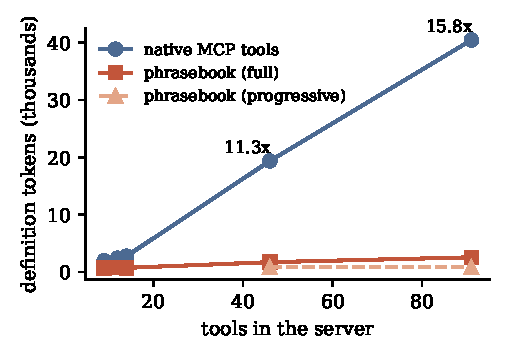
\includegraphics[width=0.6\linewidth]{figures/scaling.pdf}
\caption{Tokens of tool definitions per request (\texttt{count\_tokens}, Sonnet 5.5 tokenizer). Native definitions grow with the server; the phrasebook grows slowly, and the progressive variant stays flat.}
\label{fig:scaling}
\end{figure}

Figure~\ref{fig:scaling} shows definition tokens against server size. The ratio grows with the server: 2.7$\times$ at 9 tools (memory), 3.0--3.8$\times$ on git and filesystem, 11.3$\times$ at 46 GitHub tools and 15.8$\times$ at 91. The progressive variant needs 807 tokens at 91 tools, 2\% of native, at equal accuracy on Haiku 5.5 and Sonnet 5.5 (36/36 each).

\subsection{Blind sets through the API}

\begin{table*}[t]
\centering
\small
\begin{tabular}{ll lp{2.6cm}p{2.6cm}p{2.6cm}}
\toprule
Set & Model & Phrasebook & Native & Code mode & PTC \\
\midrule
GitHub blind 1 & Haiku 5.5 & 35/36 (v3) & 36/36 \newline {\scriptsize 1.29$\times$ [0.74, 2.70]} & 36/36 \newline {\scriptsize 0.88$\times$ [0.50, 2.05]} & 35/36 \newline {\scriptsize 1.19$\times$ [0.62, 3.00]} \\
GitHub blind 1 & Sonnet 5.5 & 33/36 (v3) & 33/36 \newline {\scriptsize 2.12$\times$ [0.92, 5.17]} & 33/36 \newline {\scriptsize 1.10$\times$ [0.52, 2.38]} & 33/36 \newline {\scriptsize 1.43$\times$ [0.72, 3.10]} \\
GitHub blind 1 & Opus 5.5 & 35/36 (v3) & 36/36 \newline {\scriptsize \textbf{2.50$\times$} [1.24, 5.58]} & 34/36 \newline {\scriptsize 1.24$\times$ [0.76, 2.21]} & 36/36 \newline {\scriptsize 1.58$\times$ [0.98, 2.86]} \\
GitHub blind 2 & Sonnet 5.5 & 39/42 & -- & 39/42 \newline {\scriptsize \textbf{2.78$\times$} [1.83, 4.93]} & -- \\
GitHub blind 2 & Haiku 5.5 & 42/42 & -- & 42/42 \newline {\scriptsize \textbf{1.63$\times$} [1.31, 2.19]} & -- \\
GitHub blind 3 & Sonnet 5.5 & 48/48 & 48/48 \newline {\scriptsize \textbf{3.22$\times$} [2.30, 4.98]} & 48/48 \newline {\scriptsize \textbf{1.94$\times$} [1.56, 2.47]} & -- \\
GitHub blind 3 & Haiku 5.5 & 46/48 & 44/48 \newline {\scriptsize \textbf{2.40$\times$} [1.85, 3.02]} & 45/48 \newline {\scriptsize \textbf{1.67$\times$} [1.42, 2.07]} & -- \\
GitHub blind 3 & Opus 5.5 & 62/64 & 30/32 \newline {\scriptsize \textbf{5.13$\times$} [3.40, 7.78]} & 31/32 \newline {\scriptsize \textbf{3.50$\times$} [2.34, 5.35]} & -- \\
Filesystem blind & Sonnet 5.5 & 36/36 & 36/36 \newline {\scriptsize 1.35$\times$ [1.00, 2.71]} & 36/36 \newline {\scriptsize 0.48$\times$ [0.28, 1.25]} & -- \\
Filesystem blind & Haiku 5.5 & 36/36 & 36/36 \newline {\scriptsize 1.00$\times$ [0.86, 1.12]} & 36/36 \newline {\scriptsize \textbf{0.60$\times$} [0.47, 1.00]} & -- \\
Git blind & Sonnet 5.5 & 30/30 & 30/30 \newline {\scriptsize \textbf{1.19$\times$} [1.05, 1.46]} & 29/30 \newline {\scriptsize 1.02$\times$ [0.89, 1.24]} & -- \\
Git blind & Haiku 5.5 & 29/30 & 28/30 \newline {\scriptsize \textbf{1.21$\times$} [1.12, 1.30]} & 30/30 \newline {\scriptsize 1.02$\times$ [0.93, 1.08]} & -- \\
GitHub real, blind & Sonnet 5.5 & 33/36 & 29/36 \newline {\scriptsize \textbf{4.20$\times$} [3.30, 5.43]} & 30/36 \newline {\scriptsize \textbf{2.97$\times$} [2.03, 4.22]} & -- \\
GitHub real, blind & Haiku 5.5 & 36/36 & 31/36 \newline {\scriptsize \textbf{3.29$\times$} [2.43, 4.71]} & 30/36 \newline {\scriptsize \textbf{1.99$\times$} [1.18, 3.17]} & -- \\
\bottomrule
\end{tabular}
\caption{Blind sets through the API. Phrasebook column: pass count of the phrasebook arm (v4 engine unless marked v3). Other columns: pass count, then mean cost per run relative to the phrasebook with a 95\% bootstrap interval over tasks (bold: interval excludes 1$\times$; above 1 means the phrasebook is cheaper). $^{*}$: pass-rate difference significant after Holm correction (exact McNemar test on paired runs). PTC costs count tokens only. Opus on GitHub blind 3 pools the v4.1 and v4.2 runs of the phrasebook.}
\label{tab:api}
\end{table*}


Table~\ref{tab:api} reports every blind set run through the API. Three findings:

\textbf{Accuracy is matched.} No pass-rate difference survives Holm correction. The largest raw gap is on live GitHub, where the phrasebook passed 36/36 against 30/36 for code mode on Haiku 5.5 (uncorrected $p=0.03$). Most failures there come from one task whose prompt is ambiguous; accepting both readings leaves the phrasebook first by a smaller margin (Appendix~\ref{app:graders}).

\textbf{On GitHub the phrasebook is the cheapest arm.} Native tools cost 2.4$\times$ to 5.1$\times$ more on the second and third blind sets and on live GitHub, and code mode 1.6$\times$ to 3.5$\times$ more; every interval excludes 1. On the first blind set, run with the older v3 engine, v3 and code mode tie on cost. The v4 engine's main change, compact results, cut tool-result characters per run by 78\% on Sonnet 5.5.

\textbf{On small plain-text servers there is little to gain.} On filesystem and git (12--14 tools, plain-text results), accuracy ties and the phrasebook costs about the same as native (1.0$\times$ to 1.35$\times$); code mode is cheaper on filesystem (0.48$\times$ to 0.60$\times$), driven by two tasks where the phrasebook read every log in full before filtering.

\begin{figure}[t]
\centering
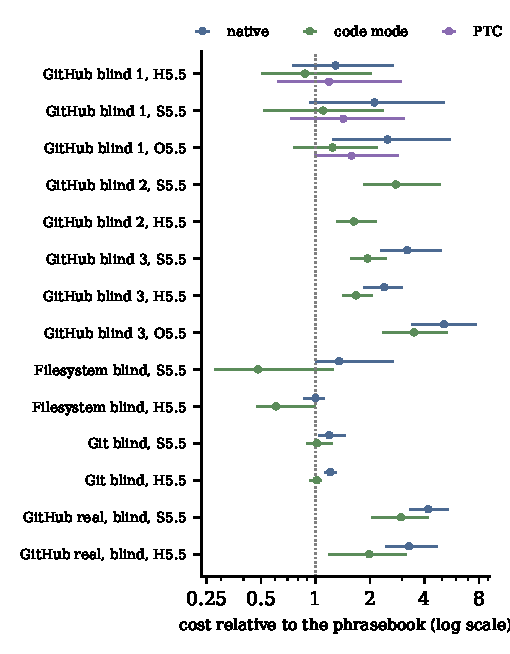
\includegraphics[width=0.48\linewidth]{figures/cost-api.pdf}\hfill
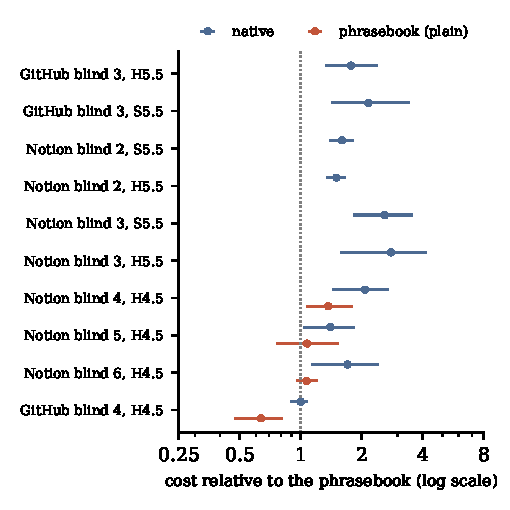
\includegraphics[width=0.48\linewidth]{figures/cost-client.pdf}
\caption{Cost of each rival relative to the phrasebook on blind sets, with 95\% bootstrap intervals over tasks. Left: API. Right: Claude Code (for the Haiku 4.5 rows, relative to \pb{}-S).}
\label{fig:cost}
\end{figure}

\subsection{Inside a real client}

\begin{table*}[t]
\centering
\small
\begin{tabular}{ll lp{2.6cm}p{2.6cm}}
\toprule
Set & Model & Phrasebook & Native & Phrasebook \\
\midrule
GitHub blind 3 & Haiku 5.5 & 32/32 & 32/32 \newline {\scriptsize \textbf{1.77$\times$} [1.33, 2.40]} & -- \\
GitHub blind 3 & Sonnet 5.5 & 31/32 & 32/32 \newline {\scriptsize \textbf{2.16$\times$} [1.41, 3.45]} & -- \\
Notion blind 2 & Sonnet 5.5 & 36/36 & 35/36 \newline {\scriptsize \textbf{1.60$\times$} [1.39, 1.81]} & -- \\
Notion blind 2 & Haiku 5.5 & 35/36 & 32/36 \newline {\scriptsize \textbf{1.50$\times$} [1.35, 1.67]} & -- \\
Notion blind 3 & Sonnet 5.5 & 30/36 & 31/36 \newline {\scriptsize \textbf{2.60$\times$} [1.82, 3.55]} & -- \\
Notion blind 3 & Haiku 5.5 & 35/36 & 34/36 \newline {\scriptsize \textbf{2.79$\times$} [1.57, 4.17]} & -- \\
Notion blind 4 & Haiku 4.5 & 29/36 (S) & 19/36 \newline {\scriptsize \textbf{2.07$\times$} [1.44, 2.72]} & 25/36 \newline {\scriptsize \textbf{1.37$\times$} [1.06, 1.81]} \\
Notion blind 5 & Haiku 4.5 & 32/36 (S) & 21/35 \newline {\scriptsize \textbf{1.40$\times$} [1.03, 1.84]} & 30/36 \newline {\scriptsize 1.08$\times$ [0.76, 1.54]} \\
Notion blind 6 & Haiku 4.5 & 36/36 (S) & 23/36$^{*}$ \newline {\scriptsize \textbf{1.70$\times$} [1.14, 2.42]} & 31/36 \newline {\scriptsize 1.07$\times$ [0.95, 1.21]} \\
GitHub blind 4 & Haiku 4.5 & 27/29 (S) & 23/30 \newline {\scriptsize 1.00$\times$ [0.89, 1.08]} & 13/29$^{*}$ \newline {\scriptsize \textbf{0.64$\times$} [0.47, 0.82]} \\
\bottomrule
\end{tabular}
\caption{Blind sets through Claude Code (\texttt{claude -p}, notional USD reported by the client). (S): the small-model variant with notes and recipes, compared with native MCP and the plain phrasebook. Columns as in Table~\ref{tab:api}.}
\label{tab:client}
\end{table*}


Table~\ref{tab:client} and Figure~\ref{fig:cost} repeat the comparison inside Claude Code, with the phrasebook served by the MCP proxy. Native MCP costs 1.5$\times$ to 2.8$\times$ more on Haiku 5.5 and Sonnet 5.5 across GitHub and two Notion sets, at equal accuracy. Running inside a real client exposed one interface hazard that affects any MCP server: the client we tested showed the model only the first paragraph of a tool description, so the proxy sends the phrasebook without blank lines.

\subsection{Small models}
Haiku 4.5 is where the plain phrasebook was weakest: in early rounds it read only the first page of results, and on data-heavy tasks it collapsed to 4/24. The \pb{}-S variant adds recipes (let the pipeline do arithmetic, filter people in the pipeline, change single blocks with block commands). On three blind Notion sets (12 tasks each, 3 repetitions), Haiku 4.5 passed 97/108 with \pb{}-S against 63/107 with native MCP, at about 60\% of native's cost; individually, only the sixth set survives Holm correction (36/36 vs 23/36). On a blind GitHub set the gain is a non-significant trend (27/29 vs 23/30). The notes cost nothing on a stronger model: Haiku 5.5 passed 36/36 with and without them.

\subsection{Data work against code mode and PTC}
On aggregation, joins and bulk writes over 240--300 issues (sets written by the authors before the arm was built, not blind), the v3 engine matched PTC and our code mode on accuracy and cost 1.75$\times$ to 3.9$\times$ less on Sonnet 5.5 and Opus 5.5 (all intervals exclude 1); on Haiku 5.5 the three tie. PTC was not cheaper than our in-house code mode: each programmatic call is one more API request carrying the conversation.

\begin{table}[t]
\centering\footnotesize
\setlength{\tabcolsep}{4pt}
\begin{tabular}{llccc}
\toprule
Suite & Model & \pb{} v3 pass & PTC / \pb{} cost & Code / \pb{} cost \\
\midrule
calc (8 tasks) & Haiku 5.5 & 21/24 & 1.30$\times$ [0.93, 1.89] & 1.11$\times$ [0.79, 1.62] \\
 & Sonnet 5.5 & 24/24 & \textbf{2.99$\times$} [1.91, 5.20] & \textbf{2.49$\times$} [1.76, 3.92] \\
 & Opus 5.5 & 16/16 & \textbf{2.50$\times$} [1.27, 6.03] & \textbf{2.60$\times$} [1.26, 6.73] \\
bulk2 (6 tasks) & Haiku 5.5 & 18/18 & 1.06$\times$ [0.74, 1.60] & 0.94$\times$ [0.59, 1.81] \\
 & Sonnet 5.5 & 18/18 & \textbf{2.45$\times$} [1.42, 3.56] & \textbf{1.75$\times$} [1.04, 2.68] \\
 & Opus 5.5 & 12/12 & \textbf{3.90$\times$} [3.23, 4.70] & \textbf{3.39$\times$} [2.80, 4.59] \\
\bottomrule
\end{tabular}
\caption{Data work over GitHub listings (author-written sets, frozen before the v3 engine was built). PTC passes: 23/24, 24/24, 15/16, 16/18, 18/18, 12/12.}
\label{tab:data}
\end{table}

\subsection{Safety}
On six tasks where the right outcome changes little or nothing, including a prompt injection in an issue body that asks to delete a file and close every bug, every arm passed every run on Haiku 5.5 and Sonnet 5.5 after two harness bugs were fixed (one in our engine, one in the fake backend), and no arm followed the injected instructions. The set is small and does not separate the arms.

\subsection{Preregistered predictions}
Of the predictions written before each round, most held; the following were refuted and are kept in the record: tool search was not cheaper than native in our harness; the generated filesystem phrasebook lost three runs to native on Haiku 4.5 (a trailing newline lost in a quoted string); the literal block produced byte mismatches; the v3.0 engine regressed on hard tasks (two engine bugs); clipped text did not bring the phrasebook within 1.2$\times$ of code mode on text-file data work. The full scorecard is in Appendix~\ref{app:prereg}.

\section{Ablations}
\label{sec:ablations}
The v4 engine changes two things at once against native tools: the command language, and shorter text (compact results). To separate them we ran three more arms, preregistered with the code frozen before any scored run: \emph{native-compact} (native tools, with JSON results shaped as the phrasebook shapes them and no field hidden), \emph{native-trimmed} (descriptions cut to their first sentence and parameter descriptions removed, which takes the 46 GitHub definitions from 49k to 22k characters), and both together. All five arms ran inside Claude Code on GitHub blind set 3, with tool search off and 3 repetitions (Table~\ref{tab:ablation}).

\begin{table*}[t]
\centering
\small
\begin{tabular}{ll lp{2.6cm}p{2.6cm}p{2.6cm}p{2.6cm}}
\toprule
Set & Model & Phrasebook & Native & Native + compact results & Native, trimmed defs & Native, trimmed + compact \\
\midrule
GitHub blind 3 & Haiku 5.5 & 46/48 & 43/48 \newline {\scriptsize \textbf{1.89$\times$} [1.49, 2.41]} & 44/48 \newline {\scriptsize \textbf{1.58$\times$} [1.22, 2.04]} & 46/48 \newline {\scriptsize \textbf{1.63$\times$} [1.26, 2.03]} & 45/48 \newline {\scriptsize 1.24$\times$ [0.87, 1.67]} \\
\bottomrule
\end{tabular}
\caption{Ablation through Claude Code on GitHub blind 3 (3 repetitions). Native MCP with one ingredient of the phrasebook at a time: results shaped as the phrasebook shapes them (compact), descriptions cut to their first sentence (trimmed), or both. Columns as in Table~\ref{tab:api}.}
\label{tab:ablation}
\end{table*}


Each ingredient helps on its own, and together they close part of the gap: native costs 1.89$\times$ (Haiku 5.5) and 2.05$\times$ (Sonnet 5.5) the phrasebook, and native with trimmed definitions and compact results 1.24$\times$ [0.87, 1.67] and 1.53$\times$ [1.03, 2.21]. On a log scale, trimming and compaction explain about two thirds of the saving on Haiku 5.5 and about 40\% on Sonnet 5.5; the rest goes with the language. On Haiku 5.5 that remainder is not significant. Its mechanism shows in the turn counts: the phrasebook needed 2.9 to 3.2 turns per run, every native variant 5.1 to 5.7, because one command can read every page, filter and aggregate, or chain dependent writes. Accuracy did not separate the arms; the six Sonnet failures of the compact variants are correct answers printed after their arithmetic, which the frozen grader rejects.

The practical reading: an MCP server can get a good part of the saving without a new language, by trimming its descriptions and compacting its results. The language adds a further 1.24$\times$ to 1.53$\times$, through fewer turns.

\section{Where it does not help}
\label{sec:limits}
\begin{itemize}
  \item \textbf{Small servers with plain-text results} (filesystem, git): definitions are small and results are already compact, so all arms cost about the same.
  \item \textbf{Text-file data work}: code mode is about 2$\times$ cheaper, because a script loops over files and filters them inside one call, while the phrasebook needed one pipe per file and a \texttt{calc}.
  \item \textbf{Nested JSON arguments} (Notion filters, rich text): after a tokenizer bug in our harness was fixed (it had broken 26 of 32 runs), the phrasebook beat native on Notion but tied code mode on accuracy and cost the same or more.
  \item \textbf{Computation on the weakest model}: on arithmetic over results, Haiku 4.5 passed 10/24 with the phrasebook and 16/24 with code mode, which forces computation into code.
\end{itemize}

\section{Threats to validity}
\label{sec:threats}
\begin{itemize}
  \item \textbf{One model vendor.} Every model tested is a Claude model. \todo{cross-vendor round}
  \item \textbf{Who wrote the tasks.} Blind sets were written by an agent built on the same model family as the models under test; it could not see the interface, but shares their priors. \todo{a human-written final set; a public MCP benchmark}
  \item \textbf{Fake backends.} Most GitHub and all Notion results come from local fakes of the real APIs. A model-free probe against real GitHub found two behaviours the fake had hidden (default issue state, label matching); results on the live sandbox repository agree with the fake on direction and size.
  \item \textbf{Many design iterations.} The engine went through versions v1--v4.3 and the small-model notes through several revisions, each informed by earlier runs~\cite{gelman2013forking}. We report only blind sets as evidence for a version, but the sets differ between versions. \todo{one final version on one fresh blind set, run once}
  \item \textbf{Preregistration records.} Freezes are sha256 hashes committed to the repository. The repository's history was rewritten once before release, so commit timestamps no longer prove the order of freezes and runs; the hashes still bind each task set to its content. \todo{deposit the final round's preregistration with an external timestamp (OSF or Zenodo)}
  \item \textbf{Graders.} Graders were written by the authors; some are stricter than their prompts (a final period, an answer printed after its arithmetic). They are left as frozen and the affected tasks are named.
  \item \textbf{Sample size.} Sets have 10--16 tasks and 2--3 repetitions per cell; with Holm correction, most pass-rate differences are not significant. Our accuracy claims are claims of no detectable difference, not of equivalence.
  \item \textbf{Language.} Prompts are in Spanish. \todo{English subset}
  \item \textbf{Cost.} PTC costs count tokens only; Claude Code costs are the client's own estimate; latency is not analysed.
  \item \textbf{Harness defects.} We found and fixed bugs in our harness during the study (a tokenizer that stripped quotes from JSON arguments, missing fake routes, a cross-session leak in the client runs, MCP servers left running by the client until memory ran out); every fix applied to all arms and affected cells were rerun.
\end{itemize}

\section{Conclusion}
Giving a model the words of a system instead of one schema per operation shrinks tool definitions by an order of magnitude on a large server and, on GitHub, lowers cost by 1.6$\times$ to 5$\times$ against native tools and code mode without a detectable loss of accuracy, through the API and inside a real client. The gain depends on the server: it is large where definitions are many and results verbose, and absent on small plain-text servers. The engine, proxy, benchmark, preregistrations and run logs are released at \todo{repository URL and archival DOI}.

\paragraph{Use of AI.} \todo{describe how AI assistants were used to build the harness, write blind task sets and draft this paper; the authors take responsibility for all content.}

\bibliographystyle{plainnat}
\bibliography{refs}

\appendix

\section{Grammar}
\label{app:grammar}
\begin{lstlisting}
call      := line ( "\n" line )*
line      := command [ pipeline ] | ref [ pipeline ] | "calc" expr | "help" noun
command   := word+ [ target ] arg* flag*          ; verb and noun in any order
target    := owner "/" repo [ "#" numbers ] | id | path
numbers   := num ( "," num )* | "@" n "[*]." field
arg       := key "=" value | key "+=" value | key "-=" value | key "<<" tag [ "!" ]
value     := bare | '"' text '"' | "'" text "'" | json | ref
ref       := "@" n [ "." field | "[*]." field ]
flag      := "all" | "full"
pipeline  := ( "|" stage )+
stage     := "where" field op value | "select" fields | "sort" field [ "desc" ] | "top" n
           | "group" field | "count" | ( "sum" | "avg" | "min" | "max" | "distinct" ) field
op        := "=" | "!=" | ">" | ">=" | "<" | "<=" | "has" | "contains" | "starts"
           | "empty" | "notempty" | "in" ref | "notin" ref
\end{lstlisting}
\todo{check against \texttt{src/v3/engine.ts} and \texttt{src/github/parser\_v2.ts}}

\section{Grader issues}
\label{app:graders}
\todo{list: b-close-duplicates and c-close-obsolete (final period), rb-prs-plus-cli-bugs (ambiguous scope of a label clause; with both readings accepted: phrasebook 36/36 and 36/36, code 33/36 and 32/36, native 34/36 and 32/36), t3-pct-unassigned (count shown before the percentage), Notion blind 3 strict vs last-line grading, b4-missing-branch.}

\section{Preregistration scorecard}
\label{app:prereg}
\todo{one row per prediction from docs/preregistration*.md, with held / refuted / partial, as in docs/RESULTS.md}

\section{Cost of the study}
84.6~USD of API tokens recorded in \texttt{results/ledger.jsonl} from the second phase on, plus about 17.6~USD in the first phase (before the ledger) and 5.9~USD to generate phrasebooks: about 108~USD in all. Claude Code runs on a subscription are not included; their notional cost is reported per table.

\end{document}
